\chapter{Deep learning and neural networks}
% What is deep learning, machine learning, AI
The concepts that fall under the definition of \textit{deep learning} become more and more popular since a wide range of tools are based on it which often achieve state-of-the-art results. Important fields are for example language problems like machine translation \cite{liu_very_2020} or speech recognition \cite{amodei_deep_2015}. Also for games like chess or Go, tools, based on deep learning are the strongest players \cite{schrittwieser_mastering_2020}. Another example for a breakthrough in recent time is a tool called AlphaFold which \glqq solved\grqq{} (according to their definition) the problem of protein folding \cite{alphafold}. It can be said that deep learning is an important topic that has made possible a large number of breakthroughs in a wide range of research areas.

The term deep learning which is a sub field of machine learning refers to the concepts of software development where a computer is not directly programmed to solve a problem, but the instructions how to find a good solution. 
The approach that falls into the area of deep learning and which is based on this concept is the training of deep neural networks (DNN), a type of artificial neural networks. DNN's are a class of non-linear functions which are characterized by a large computational graph. A typical example of a neural network (regardless if it is deep or not) is the feed-forward network. It consists of the combination (or composition) of several similar functions the so-called layers, where each is build by a combination of a linear function and a non-linearity, the so-called activation function. Each layer provides a new representation of the input which passes through them. With each layer, the representation can be developed in a way, that it finally provides a meaningful representation, with respect to a given problem. This is a very brief description of the functionality, in the following section I will explain the mathematical basics behind it and important variations of the mentioned layers. 


%The field of machine learning becomes more and more popular since a wide range of tools are based on it respectively on deep learning, a sub field of machine

%The terms machine learning refers to the concept that a machine is not given instructions directly how to solve a problem, but 

%The field of machine learning is concerned with the question of how to construct computer programs that automatically improve with experience.


%With deep learning it has been able to achieve state-of-the-art results in a variety of problems. Important fields are for example language problems like machine translation or speech recognition [CITE]. Also for games like chess or Go, tools, based on deep learning are the strongest players [CITE]. Another example for a breakthrough in recent time is a tool called AlphaFold which \glqq solved\grqq{} (according to their definition) the problem of protein folding [CITE]. It can be said that deep learning is an important topic in artificial intelligence that has made possible a large number of breakthroughs in a wide range of research areas, but how does it work and how can it be used for such a variety of problems as mentioned above. %This question will be answered in the following.

%Deep learning is about the training of deep neural networks, a class of non-linear functions which is characterized by a large computational graph. \textcolor{red}{What a comparatively large graph means is explained in the following section.} A typical example of a neural network (regardless if it is deep or not) is the feed-forward network. It consists of the combination (or composition) of several similar functions the so-called layers, where each is build by a combination of a linear function and a non-linearity, the so-called activation function. Each layer provides a new representation of the input which passes through them. With each layer, the representation can be developed in a way, that it finally provides a meaningful representation, with respect to a given problem. This is a very brief description of the functionality, in the following section I will explain the mathematical basics behind it and important variations of the mentioned layers. 

%the functionality of neural networks in general.
% What is AI, Machine learning, Deep learning
%Since both experiments contain methods of machine learning, I give a brief overview of the different methods.
%In this chapter I introduce some fundamental about the 

%\begin{figure}[ht]
%    \center
%    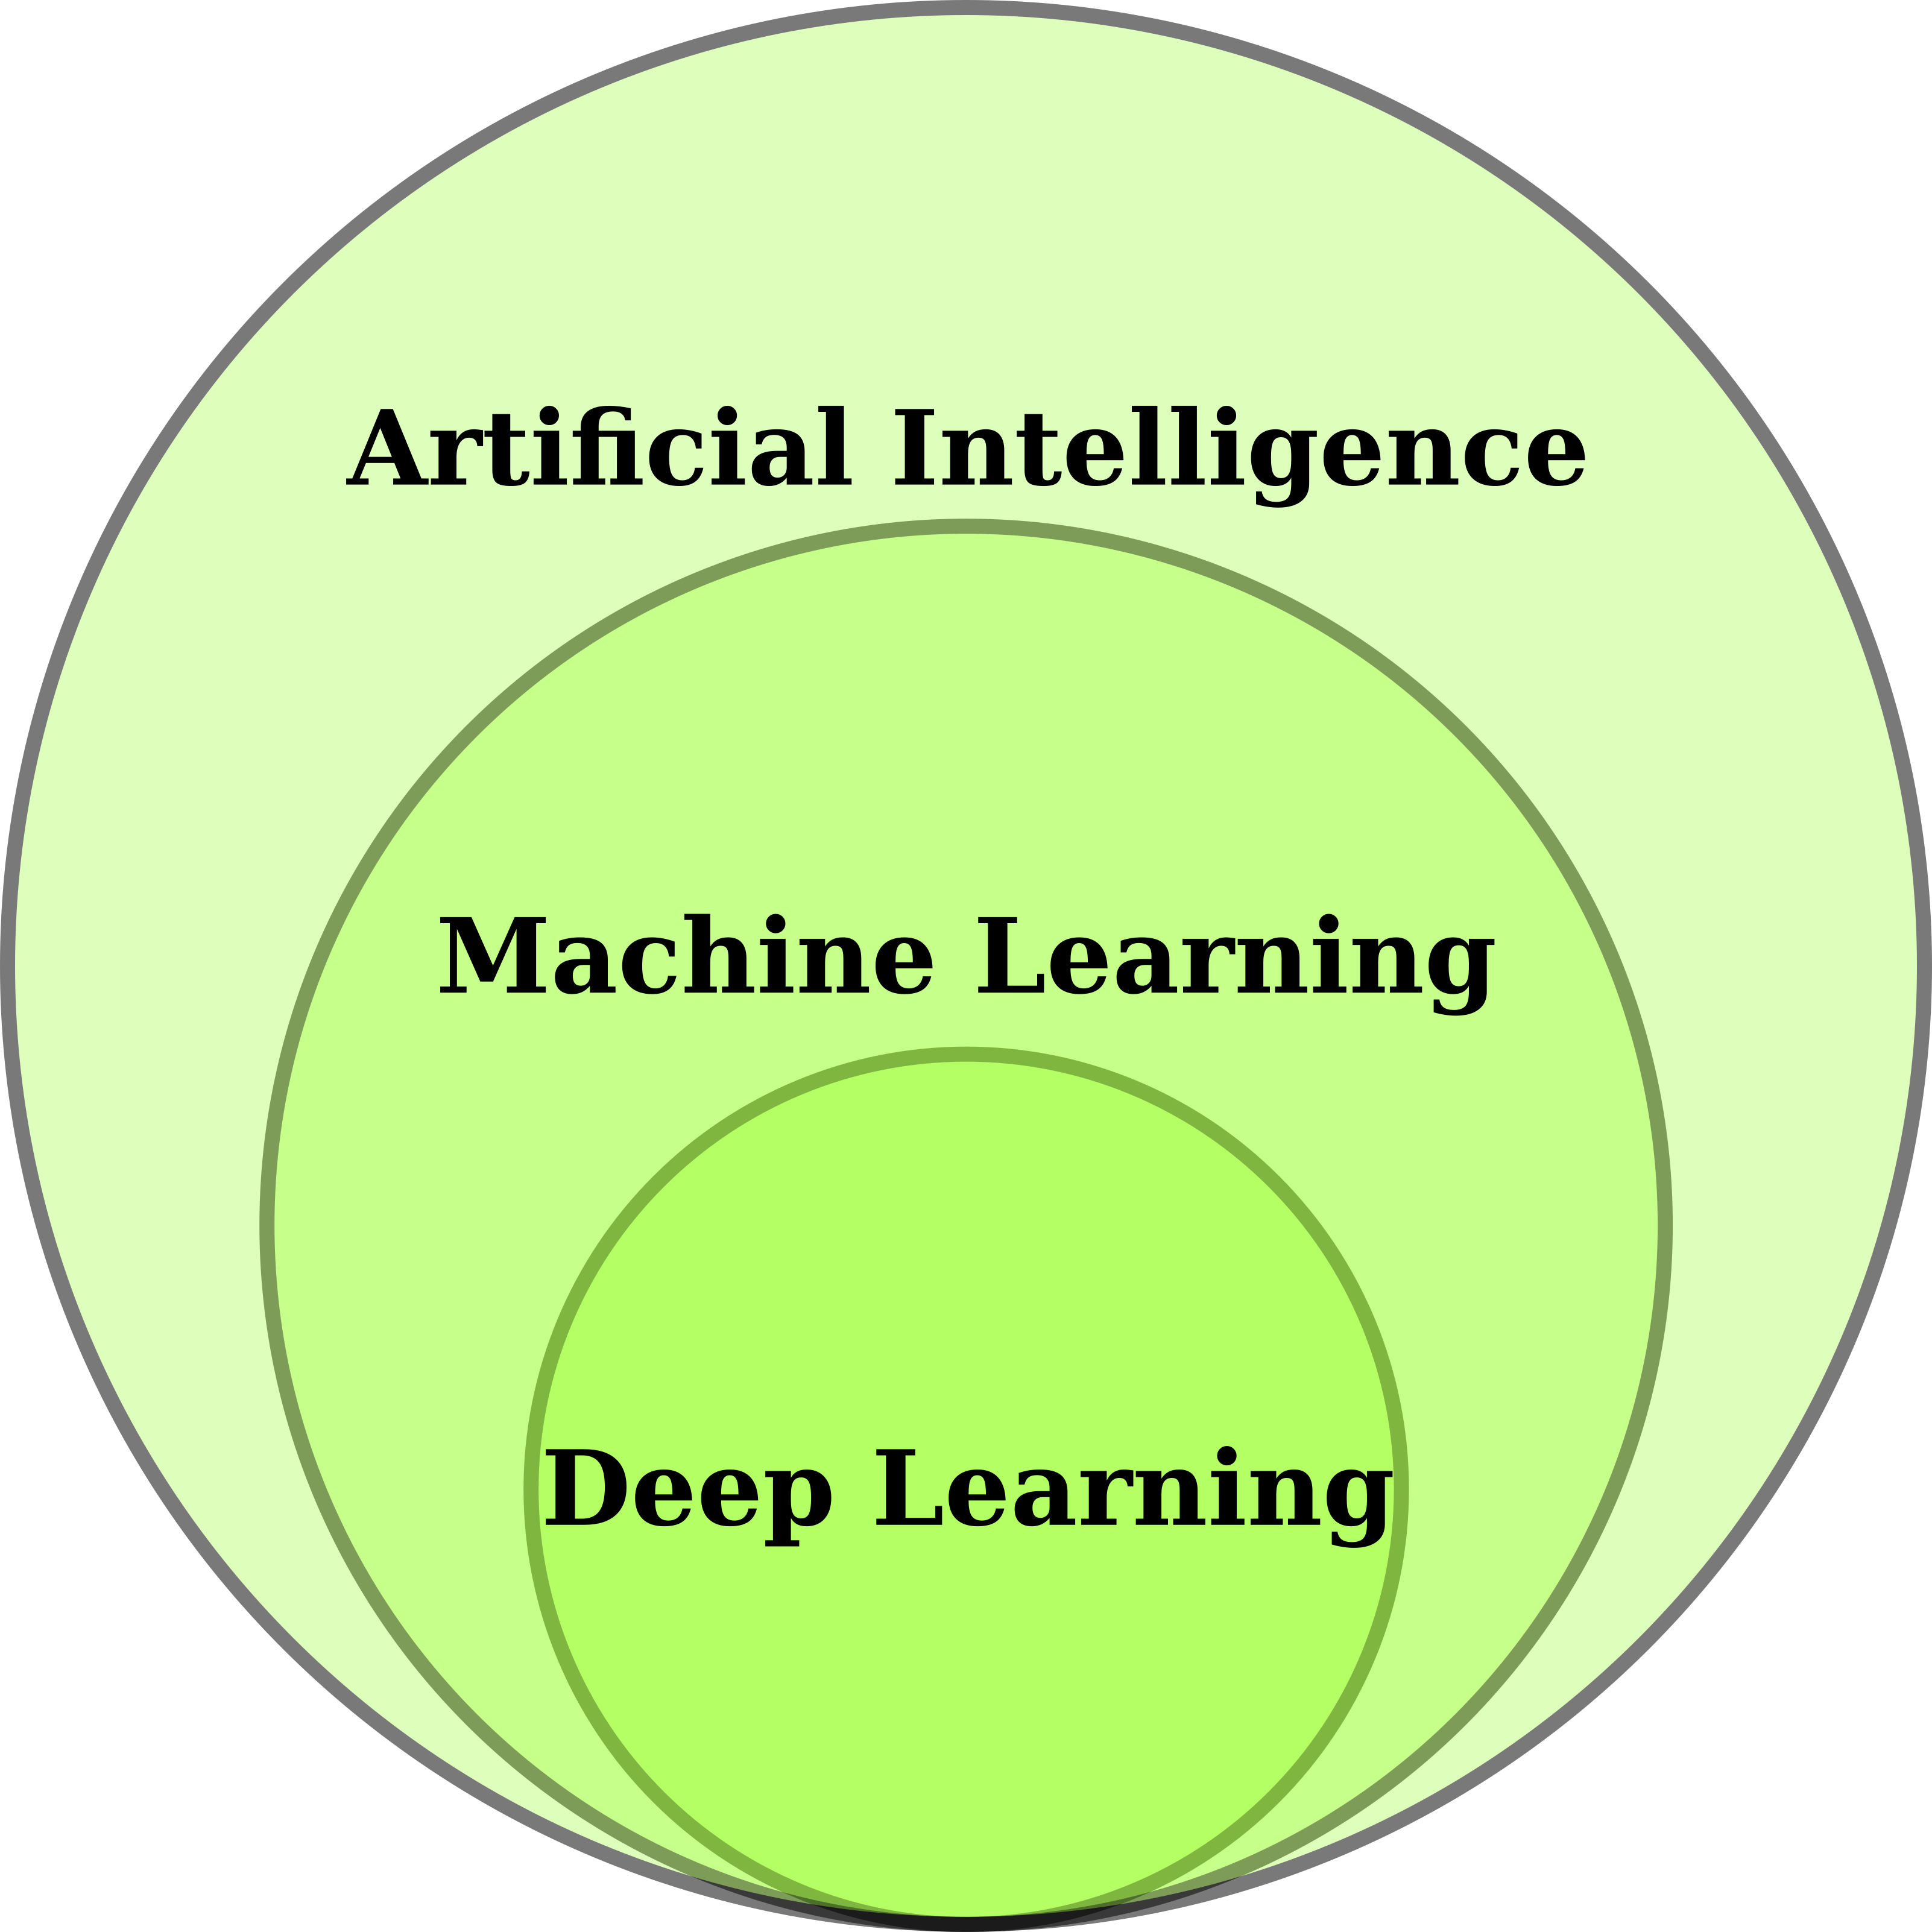
\includegraphics[width=0.6\textwidth]{figures/aimldl.png}
%	\caption{From artificial intelligence to machine learning to deep learning.}
%	\label{fig:aimldl}
%\end{figure}

%\textbf{Training}
%\textbf{Dataset}

% what is machine learning 

% Biological motivation
% Reinforcement, supervised, unsupervised, (semi-supervised)
% What are they capable of? (Some of the greatest works: Machine translation, Image classification, medizine)
% Leserorientierung: In detail which methods exactelly



\section{Artificial Neural networks}
Artificial neural networks are inspired by biological neural systems. Yet strongly simplified, the terminology is oriented on parts of the brain. A first approach for artificial neural networks was introduced by Warren McCulloch and Walter Pitts 1943 in their paper \glqq A logical calculus of the ideas immanent in nervous activity\grqq{} \cite{mcculloch_logical_1943}, where they explain their idea of a computational model which could represent mathematically how animal brains work on the scale of neurons to perform complex tasks. Their neural network is built from binary units with one or multiple binary inputs. It is able to perform simple binary classifications respectively logical computations. However, a more general description of a neuron is a based on continuous calculations, whose mathematical concepts I explain in the following.

\subsection{Mathematical computations in artificial neural networks}
The smallest functional unit of an artificial neural network is the neuron. As mathematical function $f$ it takes a number of weighted scalars and outputs the sum of them. It is a linear function which quantity is represented by a weight-vector $\textbf{w}$ and a bias $b$. The computations of a neuron are 

\begin{align}
    y=f_{\text{neuron}}(\textbf{x})\equiv\textbf{w}^T\textbf{x}+b,
\end{align}
where $\textbf{x}=(x_1,...x_n)^T\in\mathbb{R}^n$ and $b\in\mathbb{R}$.

However, a so-called layer in a feed forward neural network contains a bunch of neurons, the computation for all neurons within the linear part of it thus is written in the form

\begin{align}
    \textbf{y}=f(\textbf{x})\equiv\underline{\underline{\textbf{w}}}^T\textbf{x}+\textbf{b},
\end{align}

with the weight-matrix $\underline{\underline{\textbf{w}}}\in\mathbb{R}^{n\times m}$ and bias-vector $\textbf{b}\in\mathbb{R}^{m}$ with the number of neurons $m$. This computation builds with a so-called activation-function $A$ a single layer in a feed-forward network. Typically, activation-functions are the logistic function 

\begin{align}
    \sigma(y)=\frac{1}{1+\exp^{-y}},
\end{align}

or the rectified linear unit (ReLU-function)
\begin{align}
    \text{ReLU}(y)=\max(0,y),
\end{align}

to mention two of the most frequently used [CITE]. Finally, the computation within a single layer can be written as

\begin{align}
    \textbf{y}=A\circ f(\textbf{x}).
\end{align}

Note that the notation is point-wise, the activation-functions compute every scalar within an input-vector $\textbf{y}$ independently. In figure (\ref{fig:nn_shematic}) the analogy to a biological neural network is visualized, where the weight matrix are represented by connections between neurons and a neuron is represented by the nodes (blue circles). In this case a neural network is shown, where three layer are composed.

\begin{figure}[ht]
    \center
    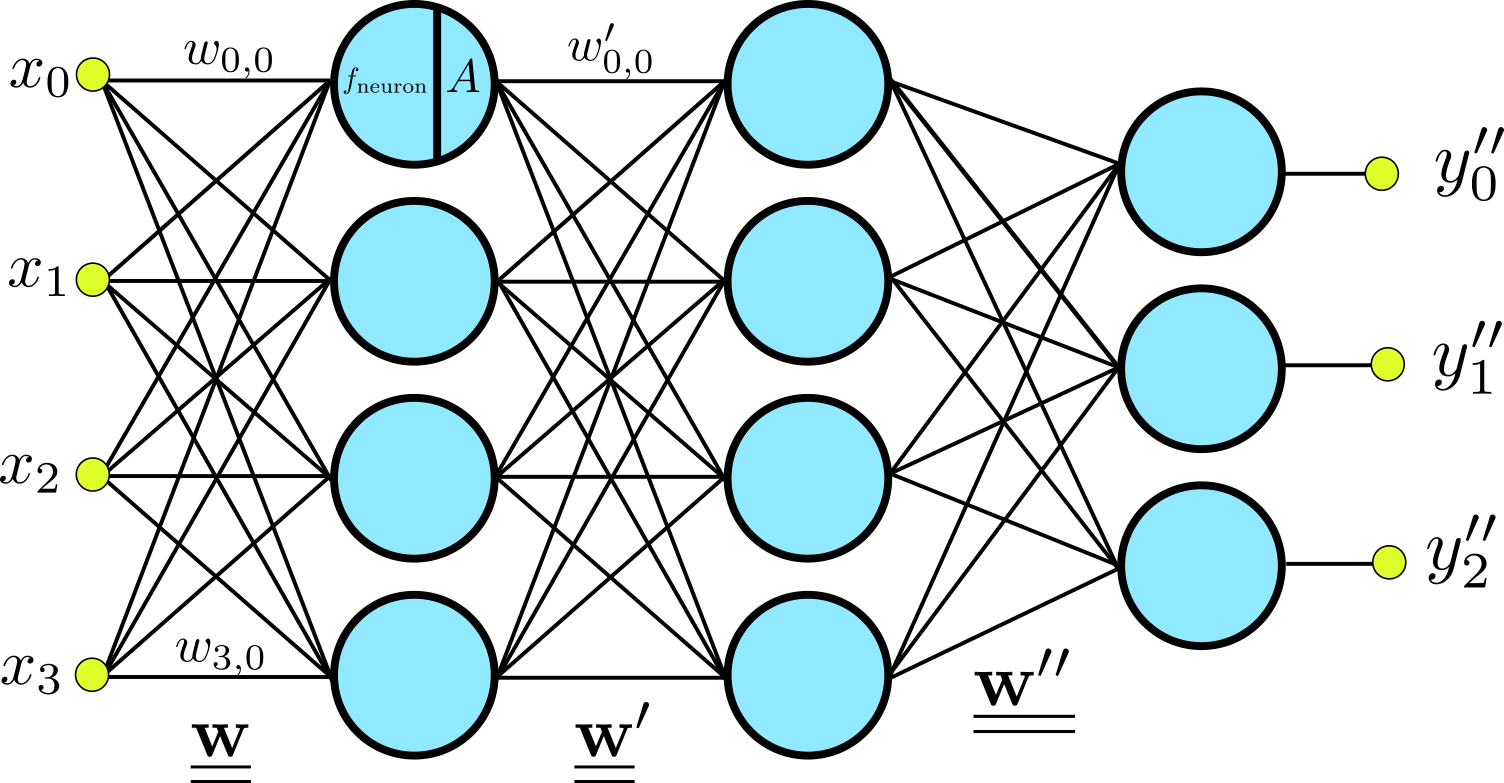
\includegraphics[width=0.8\textwidth]{figures/nn_shematic.png}
	\caption{Schematic view of the computation within a feed forward network, considerably the most simple neural network architecture.}
	\label{fig:nn_shematic}
\end{figure}

The key of a neural network is that the weight matrices and biases are adjusted in a way that the network gives a useful output $\textbf{y}$ regarding a given problem. These parameter will be adjusted in the training process whose fundamentals I introduce in the following section.

\subsection{Training of neural networks}
% What is training briefly
The search for the networks optimal parameter adjustment is called training process. The goal of training a neural network is that the network performs good on yet \textit{unseen} data when the performance is measured by a loss-function, which computes the discrepancy between predictions and the \textit{true values}. Predictions are the output of the neural network, previously noted as $\textbf{y}$ while the \textit{true values} are the aim for what the network should predict, based on a given input. Mostly, the training is a minimization process by applying a distance metric such as mean squared error to quantize the validity of the prediction.

The subject of machine learning can be roughly divided into three areas: Supervised learning, unsupervised learning and reinforcement learning.
Here an input is already assigned to a corresponding output, the relationship which the network is supposed to learn. This type of training process is called supervised learning. Since this work contains of two experiments which focus only on supervised learning, when explaining the training process, I only consider this case.
%(VORHER DEFINIEREN: Data, true values in supervised learning, prediction) 

%Usually, the data set is divided into subsets: The training-data which is used during the training process, and validation data to measure the networks performance, while this data set is not included in the training process.

\subsubsection{Optimization process}
% How does training work
Optimizer are iterative algorithms to find the optimal networks parameter which (mostly\footnote{Dependent on the loss-function, the goal could also be the maximization. Nonetheless every loss-function can be reformulated so that the training process is again a minimization task, without changing the properties of the loss function.}) minimize a loss function $L$. With each iteration, a sub set of the training data called batch is passed to the loss function, whose gradient with respect to the networks parameter $\theta$ is then used to update these parameter. The gradient calculation is performed by the backpropagation algorithm \cite{Rumelhart1986} in the parameter space. There exist a lot different optimizer respectively update-rules, from which I will explain one of the most basic one called \textit{gradient descent}, to have an idea about the general functionality. Every optimizer of this kind is as well based on an update rule including the gradient of a loss function. An update in the \textit{gradient descent} algorithm is computed according to

\begin{align}
    \theta_{\text{new}}=\theta+\eta\cdot\nabla_{\theta}L(f(X|\theta),y),
\end{align}

where $\eta$ is the learning rate, a quantity to adjust how big the network parameters $\theta$ can change within an updated. The right choice of this parameter is critical \cite{wu_demystifying_2019}. There are three types of gradient descent methods which differ in the amount of data to be passed through one iteration. If $X$ contains of one \textit{data-point}, the optimizer performs a parameter update with every single training example. In contrast there is the \textit{batch gradient descent} which calculates the gradient on the whole dataset to perform a parameter update
The third possibility is a compromise of both, where the optimizer only uses a part of the dataset which however contains more than one single example each, to perform one parameter update.

Probably the most famous optimization-algorithm in machine learning is the Adaptive Moment Estimation optimizer (Adam)\cite{adam} which is specifically designed to train neural networks. Firstly introduced in 2014 it showed big performance gains in training speed. In this work I use the same optimizer for every training process.\\

%\textbf{Loss-function}\\
%Previously denoted as $L$, the loss-function is a critical 
%During the training process, one has to face the following problems:\\

\textbf{Overfitting}\\
When training a model on a dataset, we want a loss-function to get smaller during the process according to that dataset, but as well that it can generalize what it learned from the training data on yet unseen data. A problem can appear if the model relies too much on the training data that it even considers secondary patterns like noise, which is a disadvantage for a model which should be able to generalize well. In the example in the left figure of (\ref{fig:underover}) the model predicts very well on the known data, but at the same time is not able to capture the most dominant trend which might be handled better by a regression with squared term. Overfitting can appear if the model is too complex or the model was trained for to many iterations. Staying in the example of figure (\ref{fig:underover}), the model is too complex, while a regression with squared term would perform better. \\

\textbf{Underfitting}\\
The problem of underfitting appears if the model is not capable of processing the complexity of the dataset. Reasons are if the model is not trained enough that did not learn \textit{enough} from the data, or if the model is \textit{too simple}.
An example is visualized in figure (\ref{fig:underover}, right), the model is not able to capture the main trend as well. This is due to the fact that here a linear regression was chosen as model, which is not able to handle a quadratic trend.


\begin{figure}[ht]
    \center
    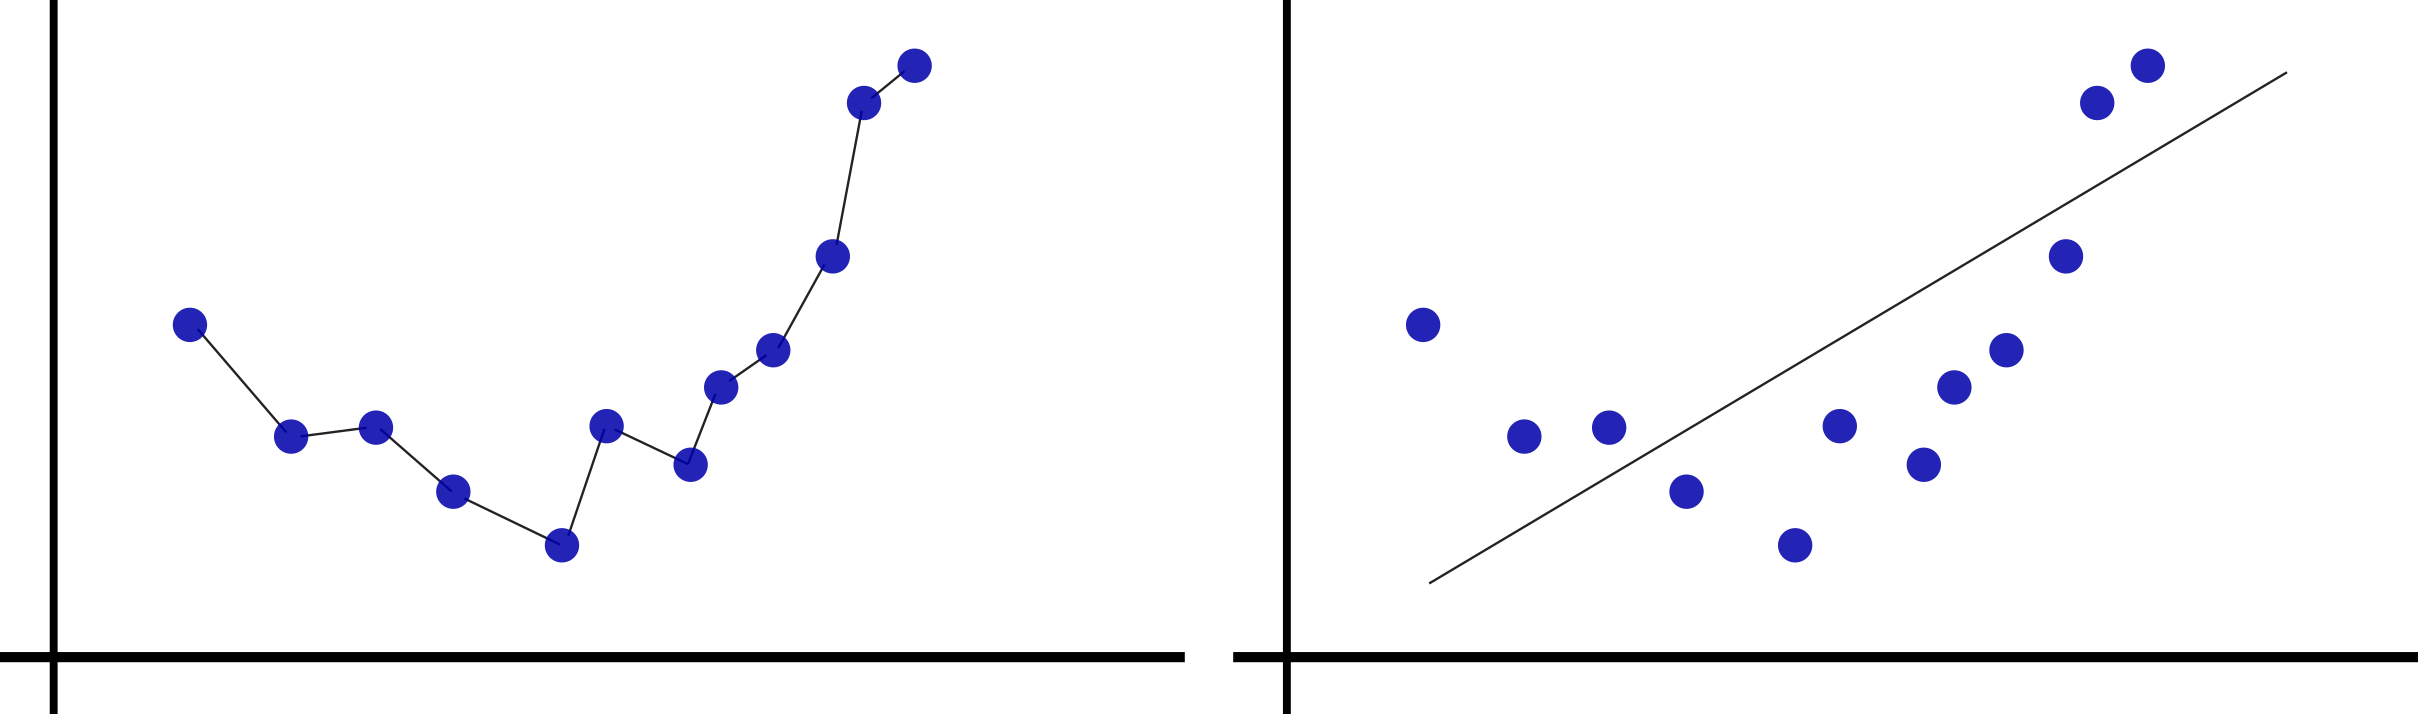
\includegraphics[width=0.99\textwidth]{figures/underoverfitting.png}
	\caption{Easy over and under}
	\label{fig:underover}
\end{figure}

To face these problem, there are a few regularization techniques which I also apply in the neural networks for in this work.

\subsection{Regularization against over- and underfitting}
The following methods to prevent overfitting and underfitting can be divided into two areas: On the one hand, I present methods that are implemented in the form of additional layers in the network (such as dropout and batch normalization), and on the other hand, there are also rules that only take effect during the training. The difference is that one method co-defines the computational graph and may have trainable parameters, while the other methods are applied during the training process.

\subsubsection{Dropout}
By ignoring a set of neurons a neural network can imitate \textit{sub networks} and is therefore able to have a dynamic architecture. The regularization technique called dropout randomly removes neurons during any execution of the network. Firstly introduced by N. Srivastava et al. \cite{srivastava_dropout_2014}, dropout helps to prevent overfitting by not allowing the network to have a rigid architecture which may be too oriented to the training data.

\subsubsection{Batch normalization}
Batch normalization can increase the stability of a neural network by normalizing the input of single layers in the neural network. It can increase the training speed with being able to handle bigger learning rates from the optimizer. Deep neural network are sensitive to the choice of initial weights and the training algorithm respectively the choice of the learning rate. Batch normalization increases the robustness with regard to the choice of these parameters \cite{ioffe_batch_2015}.

\subsubsection{Early stopping}
While the two previous regularization techniques require to be implemented with the neural network, early stopping  is a rule that takes effect during the training process. It interrupts the training process as soon as there is no improvement in the loss for the test set for a longer period, a so-called \textit{plateau}.\\


%The following regularization, which I apply does not face the over- or underfitting problem, but is regarded as 

%\subsubsection{Reduce learning rate on plateau}


\subsection{Convolutional neural networks}\label{cap:convolution}
%Intro, why good, good somewhere else, good in this work.
How neural networks possibly have been inspired by biological brains, convolutional neural networks (CNNs) might have its inspiration from the brain’s visual cortex. They are commonly designed for tasks in computer vision and have been able to achieve state-of-the-art results with models which includes convolutional operations. Examples \textit{EfficientNet} in image classification \cite{tan_efficientnet_2020} or \textit{EfficientPS} in semantic segmentation \cite{mohan_efficientps_2020}. Nonetheless, CNNs are not restricted to computer vision tasks, but also successfully used for example in \textit{ContextNet} for speed recognition \cite{han_contextnet_2020} or in natural language tasks like machine translation as in \textit{ConvS2S} \cite{edunov_classical_2018}. In this work CNNs are used to process electrocardiography signals (See chapter \ref{cap:}). However, I firstly focus on visual tasks to explain the computations behind CNNs since it is most common use case. Later in this work, instead of a 2D image as an input, a 1D ECG-signal is used as well, but the mathematical principles are the same, which can easily be transposed to a lower-dimensional case. 

\subsubsection{Kernel-convolution}
A convolutional neural network is based on the kernel-convolution. It is a discrete operation where a small matrix $W$, called kernel or filter, is passed over an image $I$ and transforms it in dependence of the kernel- and image-values. The operation is computed as 

\begin{align}
    g_{x,y}= W*I_{x,y}=\sum_{dx=-a}^a{\sum_{dy=-b}^b{W_{dx,dy}\cdot I_{x+dx,y+dy}}},
\end{align}

where $a$ and $b$ indicate the size of the kernel $W$. The function is calculated for all $x$ and $y$ on the image on which the filtered image $g$ is based on. 

\subsubsection{Multi-channel convolution} \label{cap:multichannel}
In most images, each pixel is represented by three values which define the color (red, green and blue). The convolutional operation should be able to take these three values (in the following called channels) into account. It is also important that multiple filters can be applied to the image, so that the input image and the output image have multiple channels. A more general description of the kernel-convolution with multi-channel input and output is given by

\begin{align}
    g_{i,x,y}^{\prime}= W_i^{\prime}*I_{x,y}=\sum_{j=1}^N\sum_{dx=-a}^a{\sum_{dy=-b}^b{W_{dx,dy}\cdot I_{j,x+dx,y+dy}^{\prime}}},
    \label{eq:multiinout}
\end{align}

with $N$ as number of channel within the input image (for example $N=3$ in an rgb-image).
Applying (\ref{eq:multiinout}) with every kernel $W_i^{\prime}$ in $\textbf{W}:=(W_1,...,W_M)$ gives a multi-channel output $\textbf{g}_{x,y}^{\prime}:=(g_{1,x,y},...,g_{M,x,y})$. 

\subsubsection{Valid- and same- convolution}
The equations above don't consider yet how the computation looks like at the edges when $x+dx$ or $y+dy$ exceeds the image boundaries. Two common rules are called \textit{valid} and \textit{same}. \textit{Valid}-convolution calculates only values for the respective point $(x,y)$ as far as it lies in the image, while with \textit{same}-convolution, zeros are added at the edge of the input image, so that the filtered image has the same width and height as the input. The parameter to implement these rules is called padding, it specifies the thickness of the additional margins added to the image with zeros.

\subsubsection{Strided convolution and max-pooling}
In previous equations, the kernel is only shifted with a step-size (stride) of one pixel. However, one can increase the step-size if $\textbf{g}$ should have smaller spatial dimensions. Furthermore, as consequence of a bigger stride, each pixel in $\textbf{g}$ is dependent of a bigger sub-field, the so-called \textit{receptive field} on the input image. The size of this field is important for processing spatial relationships within the image [CITE].

While \textit{stride} is a hyperparameter of the kernel-convolution operation, \textit{max-pooling} is a technique that functions as an independent layer in a neural network. It divides the input (here a 2D-image) into subsets like 2$\times$2-fields of spatial neighbouring pixels and outputs only the maximal image value of each. This technique reduces the spatial dimension of the input as well, and increases the receptive field. \\

In this work, convolution-layers are implemented within neural networks of both experiments. The first experiment applies a 1D-convolution to process through electrocardiography-signals, while in the second experiment, 2D-convolutions are used to encode spatial correlations and decode a low dimensional representation of images.

The chapter showed how convolutional neural networks process through spatial\footnote{The terminology \textit{spatial} does not necessarily refer to data points that are spatially related. It is to be understood more generally in the sense that data points, such as the pixels of an image, in the form in which they are stored (as a 2D array in this example) also contain information through their position and their neighbors.} correlations. In the next chapter I introduce recurrent neural networks, which are designed to process temporal dynamics in sequences.

\section{Recurrent neural networks}
%Intro (what problems for example)
The prominent domain for recurrent neural networks are sequence-to-sequence problems.
It is about training neural networks to convert a sequence to another sequence. A famous task in this domain is machine translation where a sequence of words in one language is transformed to another sequence of words of a different language. Other important tasks are for example speech-recognition where an encoded voice recording has to be converted into a sequence of words, or next-frame-prediction, a task to predict the future frames of a video. In each example, recurrent networks were considered as state-of-the-art, at least for a while. [CITE]

% public datasets
%A large number of famous problems are connected to public data sets, where models can be tested and compared with each other. Furthermore, several validation metrices

% Problems
A characteristic that is generally seen with sequence-to-sequence (seq2seq) problems is that the sequences are of variable length. For example, a translation-model has to be able to take a sequence with varying length of words to output a translation as a sequence with a varying length as well. Furthermore a strong translation model should be able to translate single words as well as a long sequences of hundreds of words. In this work, in the second numerical experiment (VERWEIS HIER) also faces the characteristic of variable input-output length, where a recurrent neural network is used as well.
Therefore, a key feature of machine learning models, designed for seq2seq problems, are their ability to handle sequences of different lengths. In the following, I introduce the smallest functional unit of a recurrent neural network, the \textit{recurrent unit}.

% Models
\subsection{The recurrent unit}
% Introduction
The recurrent unit is a form of neural network which is, in combination of an iterative approach, able to process through an input sequence with varying length. Recurrent neural networks (RNNs) which are built of one or multiple recurrent units (for example stacked into deep RNNs) can be regarded as a generalization of a neural network. With every iteration a \textit{hidden state}, which has a fixed dimensionality, is evolving to be dependent on every time step before. The \textit{hidden state} can be calculated, regardless of the length of the input sequence, and provides a representation of the sequence. \\

% Exact definition
The following equations are the computations within a very basic recurrent unit which builds the so called Elman network \cite{elman_finding_1990}. Given a sequence of inputs $(x_1,x_2,...,x_T)$, the hidden-state $h_t$ evolves as

\begin{align}
    h_{t}&=f_h(\textbf{W}_{x}\cdot x_t + \textbf{W}_h\cdot h_{t-1} + b_h),\notag\\
    y_t&=f_y(\textbf{W}_y\cdot h_t + b_y).\notag\\
    \label{eq:vanillarnn}
\end{align}

Furthermore it gives an output sequence $(y_0,y_1,...,.y_T)$ of the same length as the input sequence, which is taken into account in deep recurrent neural networks by stacking multiple RNNs. The functions $f_h$ and $f_y$ are activation functions like $\tanh$ or the sigmoid-function. \\

\subsubsection{Extensions}

\textbf{Bidirectional RNN}\\
Bidirectional RNNs combine the input sequence and the inversion through time of the same sequence. It can be regarded as an implementation of two independent RNNs which compute through the forward and backward direction of the input, whose output is stacked together. With this form of RNNs the output layer can combine information from the past and future and was firstly introduced by M. Schuster et al. in 1997 \cite{schuster_bidirectional_1997}.\\[1em]
\textbf{Stacked RNN}\\
RNNs can be stacked by taking the output sequence ($y_1$, ..., $y_T$) or the sequence of hidden states ($h_1$, ..., $h_T$) as input for a new RNN. Although it is not theoretically clear why stacked RNNs perform in certain tasks better than single-layer RNNs, in practise it provides a higher learning capacity \cite[p.51]{goldberg_primer_2015}.

\subsubsection{Training of recurrent neural networks}
The computation of the gradient of recurrent neural networks it is not possible by the normal backpropagation algorithm. However, there is a generalization of it called \textit{backpropagation through time} or \textit{BPTT}. The key behind this algorithm is to unfold the network through time into a feed forward network with multiple layers. Therefore the depth depends linear on the length of the input sequence. 

During training the gradient tends to vanish or explode, as firstly discovered by Hochreiter in 1991. He described it as follows:\\ \textit{With conventional \glqq Back-Propagation Through Time\grqq{} [...], error signals \glqq flowing backwards in time\grqq{} tend to either blow up (1) or vanish (2): the temporal evolution of the backpropagated error exponentially depends on the size of the weights. Case (1) may lead to oscillating weights, while in case(2) learning to bridge long time lags takes a prohibitive amount of time, or does not work at all.} \cite{kolen_gradient_2009}.\\
Within the learning algorithm gradient descent, which includes backpropagation, these difficulties are theoretically validated with any loss function \cite{bengio_learning_1994}. Various methods have been proposed to deal with the problem of vanishing and exploding gradient, whereby the most successful is the Long-short-term-memory (LSTM). Hochreiter and Schmidhuber introduced a special kind of RNN in 1997 which is able to prevent the problem of vanishing gradient.

\subsection{Long-short-term-memory}
%\textcolor{red}{LSTM networks were specially designed to learn long-term dependencies and avoid the vanishing gradient problem. The central idea is to have a recurrent edge within each cell that has a weight w = 1. This eliminates the problem of the vanishing gradient problem, as recurrent multiplication by 1 does neither diverge norconverge to zero. To still enable a LSTM to learn a process called constant error carousel controlsthe cell state from one sequential step to the next without any weights being multiplied directly. In-formation flows on two levels from one step to the next while the update of the weights is con-trolled by so-called gates. Gates use different activation functions to forward or stop the informationflow.}

LSTMs work on the same principle as RNNs by evolving a hidden state through an input sequence, but they use a different function to compute the hidden state which furthermore includes an additional state, the \textit{cell state}. With the computations in a LSTM unit it is provided that the gradient of the cell state can be unchanged through time. It is possible to process long term dependencies in a sequence more efficiently. Furthermore, a LSTM overcomes the problem of a vanishing gradient.

The calculations within a LSTM unit it given by

\begin{align}
    g_t&=\tanh\left(\textbf{W}_{cx}\cdot x_t + \textbf{W}_{ch}\cdot h_{t-1} + b_g\right), \notag\\
    i_t&=\sigma\left(\textbf{W}_{ix}\cdot x_t + \textbf{W}_{ih}\cdot h_{t-1} + b_i\right), \notag\\
    f_t&=\sigma\left(\textbf{W}_{fx}\cdot x_t + \textbf{W}_{fh}\cdot h_{t-1} + b_f\right), \notag\\
    o_t&=\sigma\left(\textbf{W}_{ox}\cdot x_t + \textbf{W}_{oh}\cdot h_{t-1} + b_o\right), \notag\\
    C_t&=f_t\circ C_{t-1}+i_t\circ g_t, \notag\\
    h_t&=o_t\circ\tanh(C_t),\notag\\
    \label{eq:lstm}
\end{align}

where $\circ$ denotes the Hadamard product, also known as pointwise-multiplication.

% introduction

% problems


% model to furthermore face these problems
\subsection{Variations and extensions}\label{cap:variationsextensions}

\subsubsection{Convolutional LSTM}\label{cap:CLSTM}
At least since the performance of convolutional neural networks (CNNs) in the ImageNet competition, it is empirically proven that CNNs are more effective and efficient in certain computer vision tasks like image classification than fully connected neural networks.
In the field of sequential learning, computer vision tasks are also formulated, such as video-classification or video-frame interpolation. However, the LSTM as implemented in (\ref{eq:lstm}) can be regarded as recurrent extension of a fully connected neural network, which is not as efficient in processing spatial correlations as a CNN. 

A LSTM with convolutional structure addresses this problem. It is better performing in certain tasks which include spatio-temporal data, as proven for example from Wu et al. for future video synthesis \cite{wu_future_2020}. Therefore, this concept is used in the second numerical experiment of this work, which also deals with the processing of spatio-temporal data.

The equations which build a convolutional LSTM are shown below:

\begin{align}
    g_t&=\tanh\left(\textbf{W}'_{cx}*x_t + \textbf{W}'_{ch}* h_{t-1} + b_g\right), \notag\\
    f_t&=\sigma\left(\textbf{W}'_{fx}* x_t + \textbf{W}'_{fh}* h_{t-1} + b_f\right), \notag\\
    i_t&=\sigma\left(\textbf{W}'_{ix}* x_t + \textbf{W}'_{ih}* h_{t-1} + b_i\right), \notag\\
    o_t&=\sigma\left(\textbf{W}'_{ox}*x_t + \textbf{W}'_{oh}* h_{t-1} + b_o\right), \notag\\
    C_t&=f_t\circ C_{t-1}+i_t\circ g_t, \notag\\
    h_t&=o_t\circ\tanh(C_t).\notag\\
\end{align}

As introduced in chapter \ref{cap:convolution}, the symbol * denotes a discrete convolution while the operator $\textbf{W}'$ are convolutional kernel. The linear operators are replaced by convolutions, that the input of a convolutional LSTM can handle a sequence of spatial data without flattening them to a vector.

\subsubsection{Spatiotemporal LSTM} \label{cap:STLSTM}
%The performance of a LSTM network depends on how good it is capable of memorizing relevant structures. 
As introduced before, a convolutional LSTM is taken into account advantages of convolutions to compute spatial correlation more efficiently. However, in a stacked convolutional LSTM, spatial correlations and temporal dynamics are not equally processed.
But these two aspects might be equally important and have to be considered equally significant in a machine learning model for spatio-temporal data. To address this problem, Y. Wang et al. introduce in their paper "PredRNN: Recurrent Neural Networks for Predictive
Learning using Spatiotemporal LSTMs" \cite{prednet} a variation of the LSTM-cell and its integration into a stacked network. They formulate the problem as follows:\\
\textit{[...] spatial representations are encoded layer-by-layer, with hidden states being delivered from bottom to top. However, the memory cells that belong to these [...] layers are mutually independent and updated merely in time domain. Under these circumstances, the bottom layer would totally ignore what had been memorized by the top layer at the previous time step.}\\

The equations for the spatio-temporal LSTM (ST-LSTM) are given by

\begin{align}\label{eq:stlstm}
    g_t&=\tanh\left(\textbf{W}'_{cx}*x_t + \textbf{W}'_{ch}* h_{t-1} + b_g\right),\notag\\
    i_t&=\sigma\left(\textbf{W}'_{ix}* x_t + \textbf{W}'_{ih}* h_{t-1} + b_i\right),\notag\\
    f_t&=\sigma\left(\textbf{W}'_{fx}* x_t + \textbf{W}'_{fh}* h_{t-1} + b_f\right),\notag \\
    C_t&=f_t\circ C_{t-1}+i_t\circ g_t,\notag\\
    g'_t&=\tanh\left(\textbf{W}''_{cx}*x_t + \textbf{W}'_{cm}* M^{l-1}_{t} + b'_g\right),\notag\\
    i'_t&=\sigma\left(\textbf{W}''_{ix}* x_t + \textbf{W}'_{im}* M^{l-1}_{t} + b'_i\right),\notag\\
    f'_t&=\sigma\left(\textbf{W}''_{fx}* x_t + \textbf{W}'_{fm}* M^{l-1}_{t} + b'_f\right),\notag\\
    M^{l}_t&=f'_t\circ M^{l-1}_t+i'_t\circ g'_t\notag\\
    o_t&=\sigma\left(\textbf{W}'_{ox}*x_t + \textbf{W}'_{oh}*h_{t-1} + \textbf{W}_{om}*M_t^l + b_o\right),\notag\\
    h_t&=o_t\circ\tanh(\textbf{W}_{1\times 1}*\left[C_t^l,M_t^l\right]).\notag\\
\end{align}

The idea behind this LSTM-adaptation is visualized in figure (\ref{fig:seq2seq}). With each layer, the spatial representation develops within an additional cell-state $M$ with each layer and is then passed to the bottom layer of the next time-step. 

\begin{figure}[ht]
    \center
    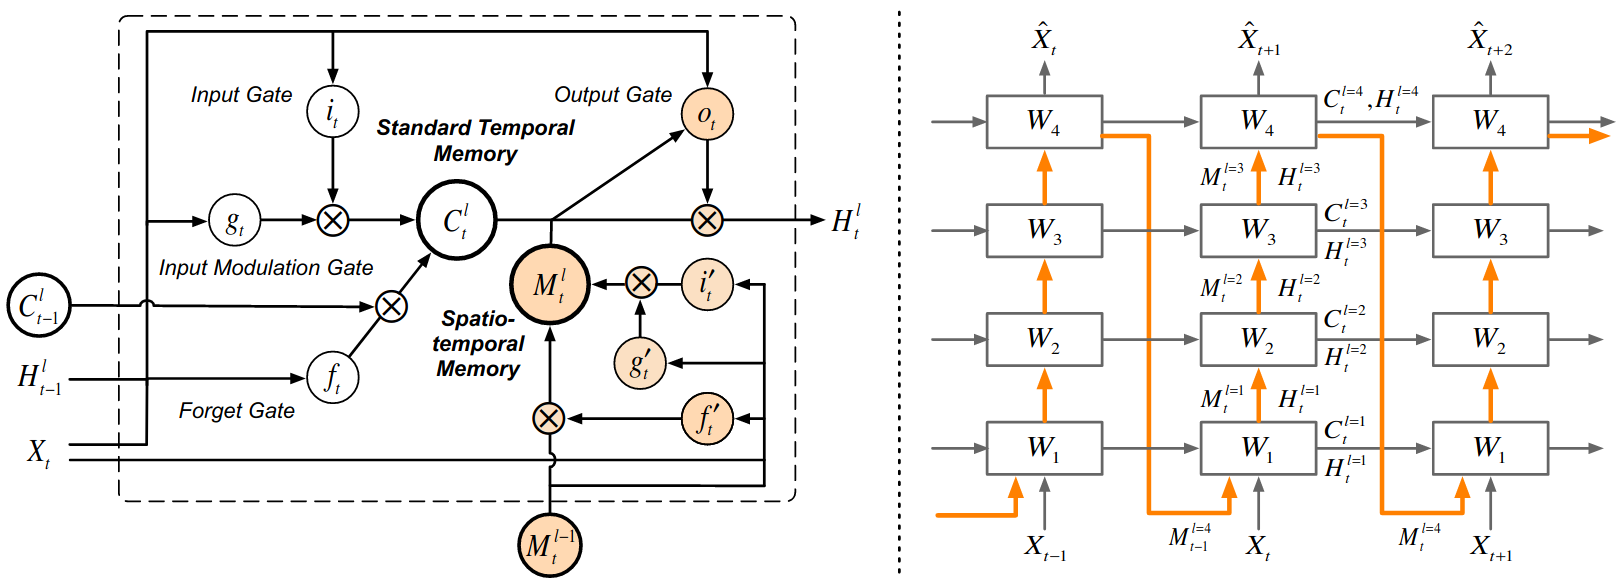
\includegraphics[width=0.99\textwidth]{figures/stlstm.png}
	\caption{Spatiotemporal LSTM, (left) the computations inside the ST-LSTM-cell, (right) the unfolded cell through time. The orange arrow marks the spatial flow through layer and time-step.}
	\label{fig:seq2seq}
\end{figure}

LSTMs are the favored implementation of recurrent networks, it is a standard to overcome general problems like vanishing gradient and learning long-term dependencies. Additionally, convolutional LSTMs or spatio-temporal LSTMs are designed to specifically face problems which occur in deep LSTMs where spatial correlation and temporal dynamics are not equally processed.

Although recurrent cells have been mentioned so far, it is not yet clear how exactly this iterative process can be used to process a sequence2sequence problem.
\section{Seq2Seq-models}\label{cap:seq2seq}
%introduction, and problems to face
A seq2seq LSTM-neural network is a type of encoder-decoder model, consisting of two LSTMs, one for encoding the sequence to a \textit{thought vector} of fixed dimension, and the other for generating an output sequence with varying length from the thought vector. Furthermore, each time-step of the input might be processed by an encoder independently, as well as the output sequence steps by a decoder as visualized in figure (\ref{fig:seq2seq}). %While there are several slight variations, which data is passed to the decoder-LSTM, in this work for the experiment in chapter 4, the same hidden-state $h_T$ (part of the thought-vector) is the input for every time-step.
% encoder-decoder models

\begin{figure}[ht]
    \center
    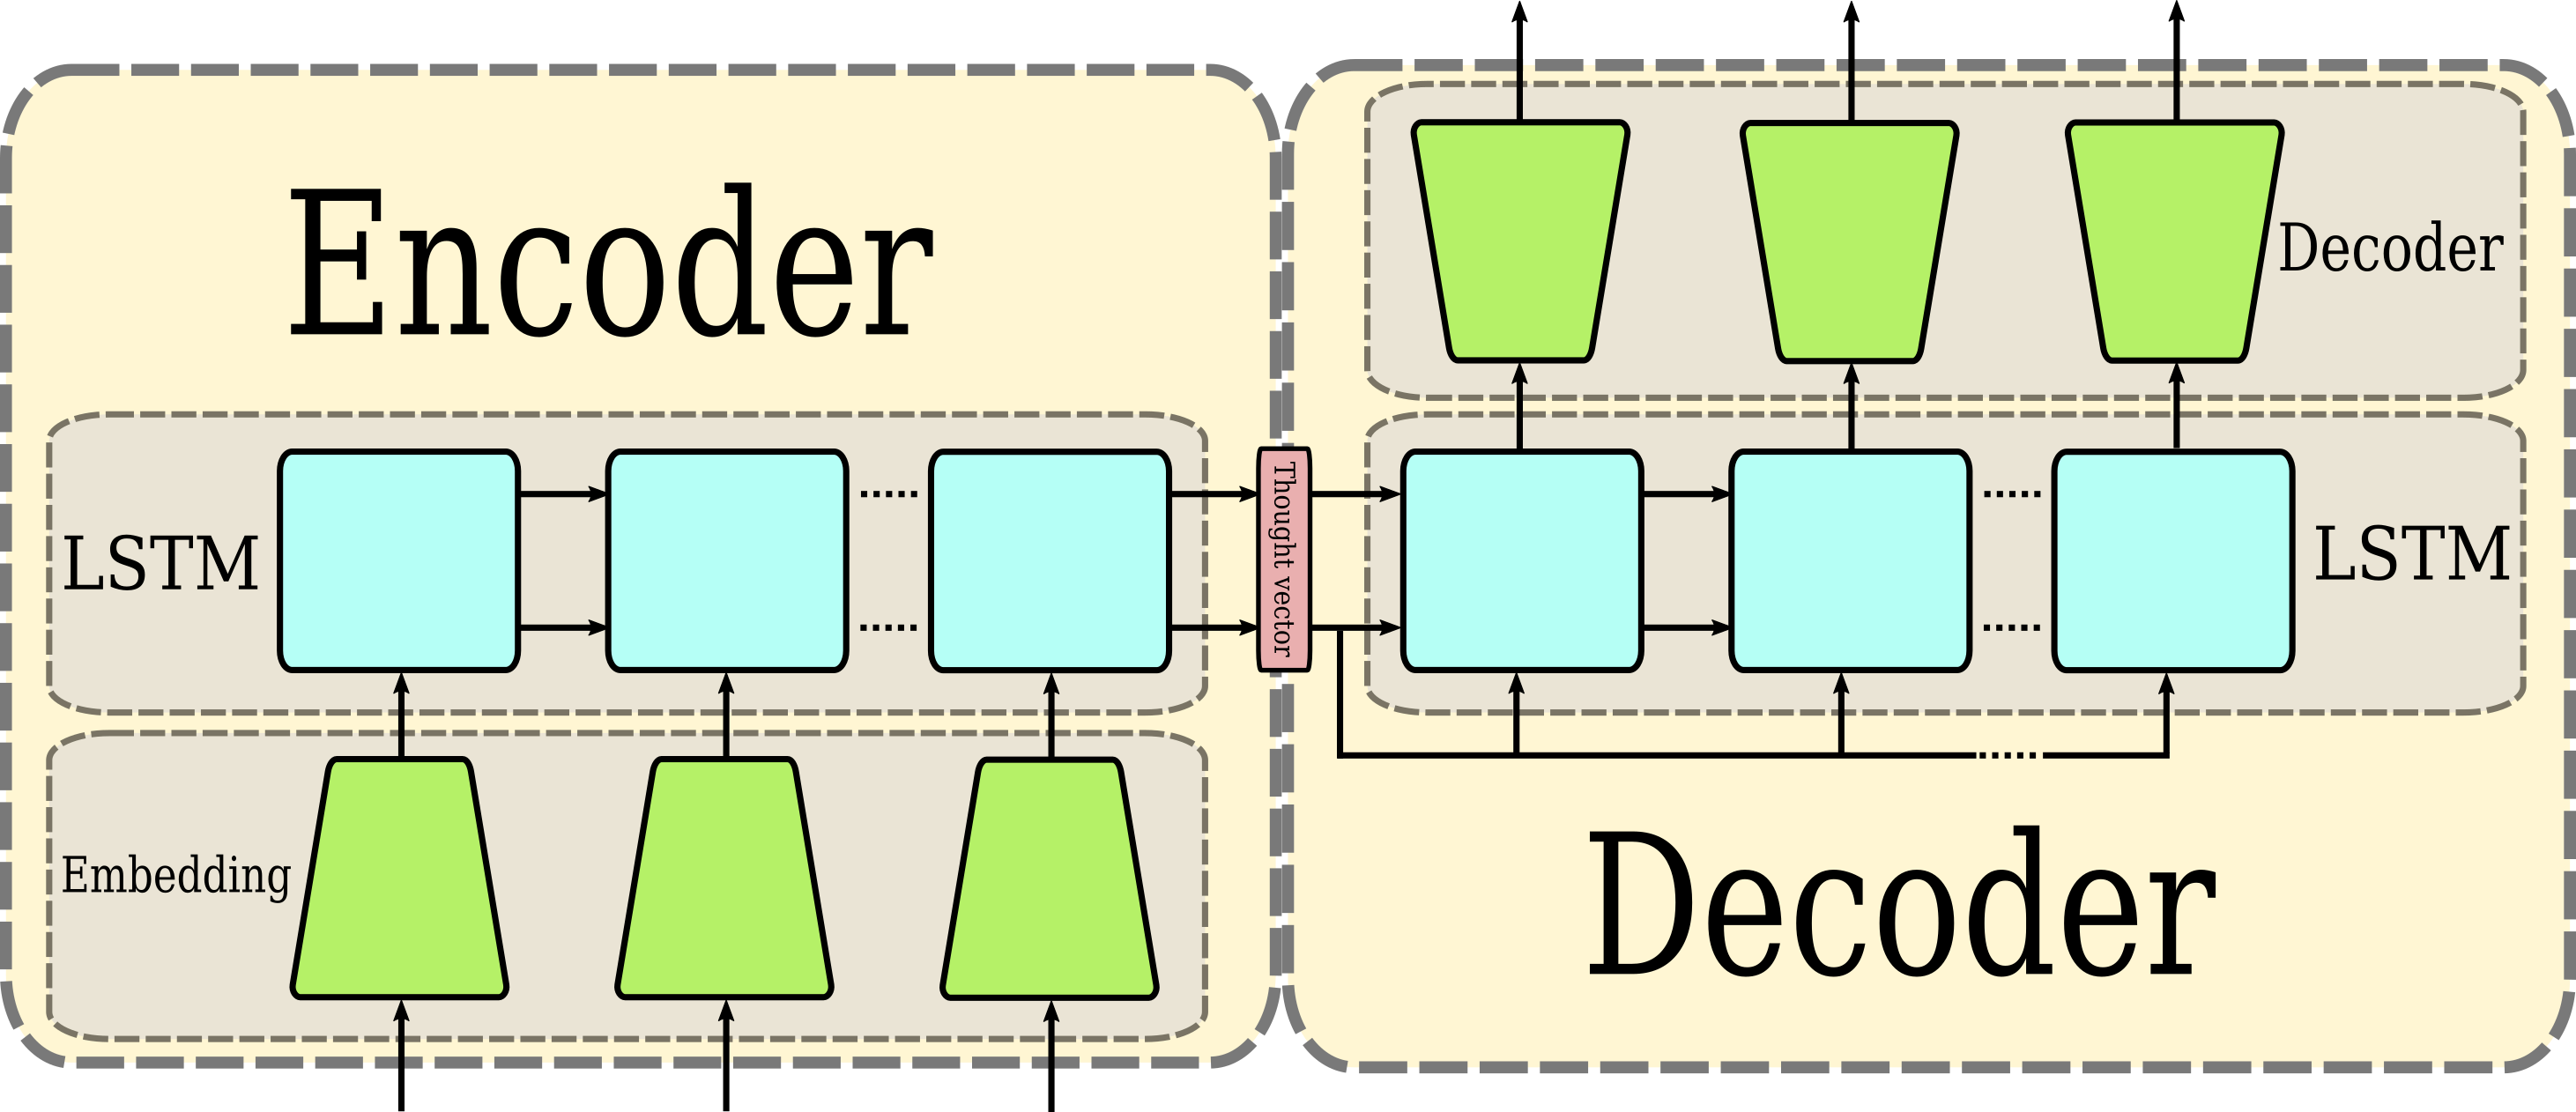
\includegraphics[width=0.99\textwidth]{figures/seq2seq.png}
	\caption{Schematic sequence to sequence model with an encoder-decoder structure.}
	\label{fig:seq2seq}
\end{figure}

%\subsection{Regularization techniques}

\section{Tools}
This chapter gives a short overview of the used software and libraries.

\subsection{Python}
\textcolor{red}{Python is a high level, general purpose programming language distributed by the Python Software Foundation (“Python – SF”). Python was first released in 1991. The current Python 3 version,which is used in this thesis, was released in 2008. It runs through an interpreter, thus python code can be run without the need to compile it. This allows for fast development and testing of code. Due to this and the huge amount of external libraries python is a widely used language in many scientific projects. It is also one of the most used language to develop NNs because it offers many powerful DL libraries, e.g. TensorFlow, Pytorch, Theano, Caffe etc. Furthermore, Python offers an almost limitless amount of other libraries useful for data preprocessing. The following three libraries wereused for this purpose:1.Numpy Numpy is a module that allows for scientific computing in Python. Its most used feature, in the context of this thesis, is the creation, editing and calculation of N-dimensional array objects (“NumPy”).}

\subsection{Keras}
\subsection{PyTorch} \label{cap:pytorch}
PyTorch \cite{pytorch}is an open-source machine learning framework, based on Torch \cite{torch}, which is the chosen API behind the majority of state-of-the-art models. By current status\footnote{According to the status in September 2020}, pytorch is the most popular framework of its kind. Together with keras (the second most used API) around 66\% of all papers based on machine learning research have used at least one of these APIs.
They support the most commonly used methods such as convolutions, LSTMs in a high abstraction.

\subsubsection{Automatic differentiation in PyTorch}

